\documentclass[sigconf,review]{acmart}

\usepackage{booktabs}

\usepackage{algorithmic}
\usepackage[tight,footnotesize]{subfigure}
\usepackage{url}

\usepackage{listings}
\usepackage[]{subfigure}
\usepackage{algorithm}
\usepackage{graphicx}
\usepackage{rotating}
\usepackage{paralist}
\usepackage{tabularx}
\usepackage{balance}
\usepackage{multirow}
\usepackage{multicol}
\usepackage{amsmath}
\usepackage{url}
\usepackage{verbatim}
\usepackage{float}
\usepackage[normalem]{ulem}
\usepackage{xspace}
\usepackage{color}
\usepackage{ifthen}
\usepackage{pifont}
\usepackage{balance}
\usepackage{mdframed}
\usepackage{hyperref}
\usepackage{booktabs}
\usepackage{colortbl}

\begin{document}


\title{Reopened Bug Prediction }
\author{Talal El Afchal}
\affiliation{
  \institution{Universit\`{a} della Svizzera italiana (USI), Switzerland}
}
\email{talal.el.afchal@usi.ch}

\begin{abstract}
% 150 to 250 words summary describing: (i) the context of the work, (ii) the performed study, (iii) the achieved results.
Reopened bugs are an undesirable problem, since they have a negative impact on the software development life cycle. In fact fixing a reopened bug generally requires double effort and time.\\
In order to predict whether a bug can be reopened after it has been fixed, we collect several informations related to the involved programmers and to the code quality and complexity, and we investigate their impact on the bug reopening prediction. \\
In this project we analyze three GitHub public repositories  \href{https://github.com/elastic/elasticsearch}{\emph{Elastic search}}, \href{https://github.com/spring-projects/spring-boot}{\emph{Spring boot}}, and \href{https://github.com/ReactiveX/RxJava}{\emph{RxJava}}. We use a machine learning tool (Weka) to classify the bug issues in $ropened$ or $\overline{reopened}$ classes. We extracted all commits and bug issues, and then we collect and create the features that we pass to Weka. These features can be grouped in three categories 1) developers experience, e.g., how many bugs did the developer fixed in the past 2) bug report, e.g., the comments and the description text  3) code quality, e.g., lines of code, cyclomatic complexity.\\
The results of our study point out that we can predict a reopen bug with $77.2\%$ \emph{precision} and $81.8\%$ \emph{recall}.
\end{abstract}

\maketitle

\section{Introduction}
%Introduction to the context of the work;
In general when a bug is detected, a \emph{bug issue} with some description is created. The developers can discuss how to solve the bug by posting their comments to the bug issue.
Once the bug is solved a commit with the fix is pushed and the bug issue is closed. At this point the programmers assume that the fix has solved the bug, and they can continue implementing other tasks on top of the fixed bug. But what are the consequences if the bug is not fixed as the programmers assumed? A reopened bug requires double effort, the programmers need to take a step back and try to understand again what the code is doing in order to locate the bug and fix it. And more than that the tasks which have been implemented can be affected by the bug and a new revision can be required. A bug reopens predictor tool which can calculate the likelihood that the bug issue can be reopened can save time and effort by suggesting the developers to add more test cases.
The bug issue and the fixing commit can tell us a lot about the bug. Our tool extracts several features as mentioned before, and they can be classified in 3 categories.
	\begin{itemize}
		\item \textbf{Developers experience}: We believe that several aspects of the developers involved in a bug issue have a big impact on the prediction. From these aspects we are interested in the developer experience in opening a bug or fixing one, and more than this we investigate if the developers have already collaborated in the past.
		\item \textbf{Bug report}: A bug report description which contains the steps to reproduce the bug, and describes the expected behavior, combined with the number of developers comments influence the bug issue understanding.
		\item \textbf{Code quality}: In many bugs reopen prediction research studies, the code complexity and quality have been ignored, but in our tool we also explore the code quality and we focus on the complexity changes before and after a fix commit.

	\end{itemize}

 %what is the importance of the project (i.e., what can we learn from it); 


 %summary of what has been done; summary of the achieved results.
 In this study we select three projects written in Java from the GitHub repositories. \href{https://github.com/elastic/elasticsearch}{\emph{Elastic search}}, \href{https://github.com/ReactiveX/RxJava}{\emph{RxJava}}, and \href{https://github.com/ReactiveX/RxJava}{\emph{RxJava}}. We found 5432 reopened bugs and 229 which are not reopened.


\section{Related Work}
There are two papers closely related to our research. Zimmermann et al. \cite{Zimmerman:reopen} analyze and categorize reopened bugs in the Microsoft Windows operating systems Windows Vista and 7, and he collected 394 developers feedback in order to understand the important factors that causes bug reopens. Zimmermann et al. main focuses was to investigate the different reasons for bug reopening.\\
On the other hand Shihab et al.\cite{Shihab:wcre} analyze work habits, bugs report, and other features to figure out which factors influence a bug reopening and a reopened bug prediction model using decision trees were built. Shihab et al. found that the comment and description texts, and time to resolve the bug, were the leading factors that caused bug reopening. \\
Our studies differ from Zimmermann et al. since we study an open source data and our main focus is to predict a bug reopening, where Zimmermann et al. main focuses stopped at understanding the factors that cause a reopening bug.\\
And our study complements Shihab et al.\cite{Shihab:wcre} since we add more features, as the code complexity and the code quality in order to predict a bug reopening, and these features are not taken in consideration in Shihab et al. work. Our study differs also in how we process the comment and description features, where we try to understand if the steps to reproduce the bug and the expected behavior are present, instead of applying correlation coefficient algorithm as Shihab et al. did.


\section{Study Design}
In this work we measure the performance of our reopens predictor.
\begin{itemize}
\item \textbf{RQ}: \emph{To what extent is it possible to predict reopened bugs?}
\end{itemize}



\subsection{Context Selection}
%What are the objects (systems) of the study? Justify your selection (i.e., why these objects?)
In order to answer our research question, we start searching on Git-hub platform the Java repositories which contain issues with \emph{bug} label. Since in Git-hub there is no way to get directly the number of reopened bugs, we had to send a request to get the event of each bug issue to understand if it is reopened or not. This procedure requires a lot of time, thus we decide to select three repositories with a high number of bug issues which increase the probability of finding reopened bugs. We found the following three Git-hub public repositories: \href{https://github.com/elastic/elasticsearch}{\emph{Elastic search}}, \href{https://github.com/spring-projects/spring-boot}{\emph{Spring boot}}, and \href{https://github.com/ReactiveX/RxJava}{\emph{RxJava}}.\\
In these repositories both issues and commits are available on the Git-hub platform, which is an important fact, since we analyze both of them and we need to link the bug issue to the fix commit. Having them on the same platform is an advantage.\\
These repositories are Java repository and we decide to analyze only projects written in Java since we calculate the CK metric by using the  \href{https://github.com/mauricioaniche/ck}{\emph{mauricioaniche}} library\footnote{https://github.com/mauricioaniche/ck}, which calculates the CK metric only for Java files.


\subsection{Data Extraction Process}
%How did you collect the data needed for your study? Carefully explain each step.
 We apply the same procedure on each repository to extract data. The first step is to get all the issues (closed and opened) and we filter the one with a \emph{bug} label.
 For each bug issue we extract the information we are interested in. The list of information is shown in Table\ref{table:issues}. \\In the next step we check if the developer mentioned how to reproduce the bug, and it is done by looking if one of the words \{\textbf{step},  \textbf{can}\}, and one the words  \{\textbf{reproduce}, \textbf{recreate}, \textbf{observed}\}  are present in the bug description. We also check if the programmer mentioned the expected behavior, and it is done by looking if one of the words \{\textbf{should},  \textbf{must}\}, and one the  words  \{\textbf{behavior}, \textbf{instead of}\} are present in the bug description. The last sept is to count the number of words present in the description and the number of developers involved in the discussion comments.\\
 We clone the repository and as a first step we extract the log file which contains the \emph{commit sha}, \emph{commit message}, \emph{author}, \emph{commit date}, and the \emph{modified files}. In the next step we map each fixing commit to the bug issue. To map a fix commit to a bug issue it has to satisfy all the following rules :
  \begin{itemize}
 	\item The commit date must be earlier than the bug issue closing date.
 	\item The commit date must be after the bug issue opening date.
 	\item The commit message has to contain the bug issue number.
 	\end{itemize}
These rules were very strict and we were able to map a very small number of reopened bugs, therefore we decide to make our mapping rules more flexible and we modify the rule \emph{The commit message has to contain the bug issue number}; to \emph{The commit message has to contain the bug issue number $\parallel$ the developer who closed the bug issue has pushed the commit}. Now that we have extracted all the information from the commits and bug issues, we can extract the social features which are shown in Table \ref{tabel:social}.\\ 

\begin{itemize}
  \item{\textbf{OpenerCommitExperience}: We calculate the number of commits that the developer did before opening the bug issue.
  }
  \item{\textbf{OpenerFixingExperience}: We calculate the number of bugs that the developer fixed before opening the bug issue.
  }
  \item{\textbf{FixerCommitExperience}: We calculate the number of commits that the developer who fixed the bug did before fixing the bug issue

  }
  \item{\textbf{FixerFixingExperience}: We calculate the number of bugs that the developer fixed before fixing the bug issue.
  }
\newpage
  \item{\textbf{SocialStrength}: For each issue we create all pairs of developers that took part of the issue discussion, and we get the social strength by 
     calculating the number of programmers that collaborates before and we divide it by the total number of programmers that is taking part of the issue discussion.
  }
\end{itemize}



\begin{table}[h]
\caption{List of extracted informations from issues} \label{table:issues}
\begin{tabular}{lll}
\hline
\hline
\multicolumn{1}{c}{Information}
& \multicolumn{1}{c}{Type}
&	\multicolumn{1}{c}{Description}    \\    

\hline
   IssueId & String & The issue id \\     
    Number & String & The issue number \\
    Title & String &The issue title \\
    Description & String &The issue description \\

    CommentAuthor & String &The comment author \\
    CommentDate & String & The comment date \\
    CommentText & String &The comment text \\
    OpenedBy & String & The developer who opened the issue \\
    OpenedOn & Numeric & The date of issue opening \\

    Reopen & Boolean & Check is the issue is reopened \\
    ReopenOn & Numeric & The date of reopening bug \\
    ClosedOn & Numeric & The date of closing the issue \\
    ClosedBy & String & The developer who closed the issue \\

\hline
\hline
\end{tabular}
\end{table}



\begin{table}[h]
\caption{List of social features} \label{tabel:social}
\begin{tabular}{lll}
\hline
\hline
\multicolumn{1}{c}{Feature}
& \multicolumn{1}{c}{Type}
&	\multicolumn{1}{c}{Description}    \\    

\hline
   OpenerCommitExperience & Numerical & Overall experience of the \\&& developer opening the bug \\     
   OpenerFixingExperience & Numerical & Bug fixing experience of the \\&& developer opening the bug \\
   FixerCommitExperience & Numerical & Overall experience of the \\&& developer fixing the bug\\
   FixerFixingExperience & Numerical & Bug fixing experience of the \\&& developer fixing the bug\\
   SocialStrength 		 & Numerical & Number of pairs of developers \\&&who took part in the issue \\&&discussion that already \\&&collaborated in the past\\


\hline
\hline
\end{tabular}
\end{table}





As a last step we calculate: 
\begin{itemize}
\item \textbf{Readability}: Calculating the readability is done by extracting source code features (i.e. line length), that are predicative of readability, which gives us a readability score. The readability is computed on all files involved in the bug fixing and its average and median across the impacted files is computed. We can expect that fixing activities performed on files with a high score are more likely to be error-prone, thus fostering the future reopening of the bug.

\item{\textbf{Comment Density (CD)}: is $\frac{\# comment\_lines}{total \# lines}$. The code density is computed on all files involved in the bug fixing and its average and median across the impacted files is computed. We can expect that fixing activities performed on files with a low CD are more likely to be error-prone, thus fostering the future reopening of the bug.
}

\item{\textbf{$\Delta$ Complexity}: Is the $\Delta$ code cyclomatic complexity computed on all files involved in the bug fixing, and it computed before and after the bug fix commit. Its average and median across the impacted files is computed. We believe that $\Delta$ complexity influences our prediction
}
\item{\textbf{Coupling Between Objects (CBO)}: Counts the number of dependencies a class has (field declaration, method return types, variable declarations, etc). The CBO is computed on all files involved in the bug fixing and its average and median across the impacted files is computed. We can expect that fixing activities performed on files with a high CBO are more likely to be error-prone, thus fostering the future reopening of the bug.
}

\item{\textbf{Depth Inheritance Tree (DIT)}: It counts the number of ``fathers'' a class has. All classes have DIT at least 1. The DTI is computed on all files involved in the bug fixing and its average and median across the impacted files is computed. We can expect that fixing activities performed on files with a high DTI are more likely to be error-prone, thus fostering the future reopening of the bug.
}

\item{\textbf{Number Of Children (NOC)}: It counts the number of ``children'' a class has. The NOC is computed on all files involved in the bug fixing and its average and median across the impacted files is computed. We can expect that fixing activities performed on files with a high NOC are more likely to be error-prone, thus fostering the future reopening of the bug.
}

\item{\textbf{Number Of Fields (NOF)}: It counts the number of fields in a class. The NOF is computed on all files involved in the bug fixing and its average and median across the impacted files is computed. We can expect that fixing activities performed on files with a very high NOF are more likely to be error-prone, thus fostering the future reopening of the bug.
}

\item{\textbf{Number Of Public Fields (NOPF)}: It counts only the public fields. The NOPF is computed on all files involved in the bug fixing and its average and median across the impacted files is computed. We can expect that fixing activities performed on files with a high NOPF are more likely to be error-prone, thus fostering the future reopening of the bug.
}

\item{\textbf{Number Of Static Fields (NOSF)}: It counts only the static fields. The NOSF is computed on all files involved in the bug fixing and its average and median across the impacted files is computed. We believe that NOSF can influences our prediction.
}

\item{\textbf{Number Of Methods (NOM)}: It counts the number of methods. The NOM is computed on all files involved in the bug fixing and its average and median across the impacted files is computed. We can expect that fixing activities performed files with a very high NOM are more likely to be error-prone, thus fostering the future reopening of the bug.
}

\item{\textbf{Number Of Public Methods (NOPM)}: It counts only public methods. The NOPM is computed on all files involved in the bug fixing and its average and median across the impacted files is computed. We We believe that NOPM influences our prediction.
}

\item{\textbf{Number Of Static Methods (NOSM)}: It counts only static methods. The NOSM is computed on all files involved in the bug fixing and its average and median across the impacted files is computed. We believe that NOSM influences our prediction.
}

\item{\textbf{Number Of Static Invocations (NOSI)}: It counts the number of invocations to static methods. It can only count the ones that can be resolved by the JDT. The NOSI is computed on all files involved in the bug fixing and its average and median across the impacted files is computed. We believe that NOSI influences our prediction.
}

\item{\textbf{Response For A Class (RFC)}: It counts the number of unique method invocations in a class. The RFC is computed on all files involved in the bug fixing and its average and median across the impacted files is computed. We believe that NOSI influences our prediction.
}

\item{\textbf{Weighted Methods Complexity (WMC)}: Is the sum of the complexities of all class methods. The complexity is computed 
by using the cyclomatic complexity (i.e., the number of linear independent paths in the code). WMC is computed on all files involved in the bug fixing and then its average and median across the impacted files is computed. One could expect that fixing activities performed on very complex files are more likely to be error-prone, thus fostering the future reopening of the bug.}

\item{\textbf{Lines Of Code (LOC)}: It counts the lines of code, ignoring empty lines. LOC is computed on all files involved in the bug fixing and then its average and median across the impacted files is computed. One could expect that fixing activities performed on files with a large number of LOC are more likely to be error-prone, thus fostering the future reopening of the bug.
}


\item{\textbf{Lack Of Cohesion Of Methods (LCOM)}: LCOM is computed on all files involved in the bug fixing and then its average and median across the impacted files is computed. We believe that LCOM influences our prediction.
}

\end{itemize}

\newpage

\begin{table}[h]
\caption{All features} \label{weka:features}
\begin{tabular}{lll}
\hline
\hline
\multicolumn{1}{c}{Feature}
& \multicolumn{1}{c}{Type}
& \multicolumn{1}{c}{Description}    \\  
\hline  
  StepToReproduce     & Boolean & Step to reproduce is mentioned \\
  ExpectedBehavior    & Boolean & Expected behavior is mentioned \\
  DescriptionLength   & Numerical & The description words count\\
  Commenters\#    & Numerical & Number of programmers who \\&& has post a comment \\

   OpenerCommitExp & Numerical & Overall experience of the \\&& developer opening the bug \\     
   OpenerFixingExp & Numerical & Bug fixing experience of the \\&& developer opening the bug \\
   FixerCommitExp & Numerical & Overall experience of the \\&& developer fixing the bug\\
   FixerFixingExp & Numerical & Bug fixing experience of the \\&& developer fixing the bug\\
   SocialStrength      & Numerical & Number of pairs of developers \\&&who took part in the issue \\&&discussion that already \\&&collaborated in the past\\

   LOCPreFix      &Numerical& Line of code before the fix\\
   $\Delta$complexity   &Numerical& $\Delta$ Cyclomatic complexity\\
   Readability      &Numerical& Code readability\\
   CD           &Numerical& Code density\\

   
   CBO &Numerical& Coupling between objects \\

  DIT &Numerical& Depth Inheritance Tree \\

NOC &Numerical&  Counts the number of children \\&&a class has\\

NOF &Numerical& Counts the number of fields \\&&in a class\\

NOPF&Numerical& Counts only the public fields\\

NOSF&Numerical& Counts only the static fields \\

NOM &Numerical& Counts the number of methods \\

NOPM &Numerical& Counts only the public methods \\

NOSM &Numerical& Counts only the static methods \\

NOSI &Numerical& Counts the number of \\&& invocations to static methods\\

RFC &Numerical& Counts the number of unique \\&&method invocations in a class\\

WMC &Numerical& It counts the number of branch \\&&instructions in a class\\

LOC &Numerical& It counts the lines of count, \\&&ignoring empty lines\\

LCOM &Numerical&Lack of Cohesion of Methods \\

   Reopened        & Boolean &  The is reopened or not\\
  

\hline
\hline
\end{tabular}
\end{table}

  
\newpage
\subsection{Analysis Method} 

% Explain how the collected data has been analyzed to answer the research questions (e.g., which descriptive statistics have been computed, data visualization, statistical tests, effect sizes, etc).

The collected data in Table \ref{weka:features} is passed to a data mining software (\emph{Weka}) which applies the \emph{RandomForest} machine learning algorithm, with 10 \emph{folds Cross-validation} technique. \emph{Weka} outputs the \emph{accuracy}, \emph{precision}, \emph{recall} and \emph{F-measure} of our prediction. Figure \ref{fig:j48} shows a Weka's tree example.


\[Accuracy = \frac{\text{Number Of Correct Classifications}}{\text{All Classifications}}\]
\[Precision =  \frac{\text{True Positive}}{\text{True Positive + True Negative}}\]
\[Recall = \frac{\text{True Positive}}{\text{True Positive + False Negative}}\]  
\[\text{F-measure} = 2 . \frac{\text{Precision . Recall}}{\text{Precision + Recall}}\]


But since the number of reopened bugs is too small compared to the not reopened ones, as we can see in Table \ref{tab:linked} is causing an imbalance problem. Our approach is to explore three different sampling techniques.
\begin{enumerate}
\item {We select a set which contains all reopened bugs and we select randomly a set with same size which contains the not reopened bugs. We repeat this step 10 times which generate 10 different not reopened bugs sets, we pass the reopened bugs set and each of the not reopened bugs sets to \emph{Weka} which gives us 10 predictions. As a last step we calculate the \emph{average, median} and the \emph{standard deviation}. The result is shown in Table \ref{table:undersampling100}} 

\item{Instead of selecting 2 sets with the same size, the not reopened bugs set will be twice bigger than the reopened bug set. As we did previously, we create 10 sets and we calculate the \emph{average, median} and the \emph{standard deviation}. The result is shown in Table \ref{table:Undersampling200}}

\item{We do the same steps that we did in point (2) with one difference, we do an oversampling where we duplicate the set of reopened bugs by creating artificial samples with similar features of the original ones. The result is shown in Table \ref{table:Oversampling}} 
\end{enumerate}

In all three sampling techniques we measure the \emph{standard deviation} to check if the result is affected by how we choose the random samples.


\begin{table} [h]
\caption{Number of $Reopened$ and $ not Reopened bugs$} \label{tab:linked}
\begin{tabular}{lll}
\hline
\hline
\multicolumn{1}{c}{}
& \multicolumn{1}{c}{$\overline{Reopened}$} 
& \multicolumn{1}{c}{$ Reopened$}    \\    

\hline
ElasticSearch      & 4019 & 105     \\
Linked        &\textbf{1795} &\textbf{42}\\ 
\hline
Rx            & 531 & 12     \\
Linked        &\textbf{259} &\textbf{7}\\
\hline
Spring          & 882 & 112     \\
Linked        &\textbf{428} &\textbf{42}\\
\hline
\hline
Total       & 5432 & 229 \\
Total linked    & \textbf{2482} & \textbf{91} \\
\hline
\hline
\end{tabular}
\end{table}
 
 \newpage

\begin{table}[h]
  \caption{Undersampling 100-100} \label{table:undersampling100}

    \begin{tabular}{llll}
    \hline
    \hline
    \multicolumn{1}{c}{}
    & \multicolumn{1}{c}{Average}
    & \multicolumn{1}{c}{Median}        
    &   \multicolumn{1}{c}{Std Dev}\\
    \hline
    Accuracy      & 0.665 & 0.645 & 0.041     \\
    \hline
    Precision-$\bar{R}$  &0.664   &0.655  & 0.038       \\
    Recall-$\bar{R}$  &0.667  &0.659  &0.052\\
    F-Measure-$\bar{R}$    & 0.666  &0.648  &0.043      \\
    \hline
    Precision-R          & 0.667  &0.648  &0.044 \\
    Recall-R & 0.662 & 0.67 &0.042 \\
    F-Measure-R    & 0.664  &0.656  &0.04\\
    \hline
    \hline
    \end{tabular}

  \end{table}
  
  \begin{table}[h]
  \caption{Undersampling 200-100} \label{table:Undersampling200}
    \begin{tabular}{llll}
    \hline
    \hline
    \multicolumn{1}{c}{}
    & \multicolumn{1}{c}{Average}
    & \multicolumn{1}{c}{Median}        
    &   \multicolumn{1}{c}{Std Dev}\\
    \hline
    Accuracy      & 0.676 &0.673 &0.023    \\
    \hline
    Precision-$\bar{R}$  &0.718 &0.718 &0.014     \\
    Recall-$\bar{R}$  &0.849 &0.846 &0.024\\
    F-Measure-$\bar{R}$    & 0.778 &0.776 &0.016\\
    \hline
    Precision-R          & 0.525  &0.517  &0.058\\
    Recall-R & 0.333 &0.335 &0.040\\
    F-Measure-R    &0.407 &0.408  &0.043\\
    \hline
    \hline
    \end{tabular}
  \end{table}


  \begin{table}[h]
  \caption{Oversampling 100-100} \label{table:Oversampling}
    \begin{tabular}{llll}
    \hline
    \hline
    \multicolumn{1}{c}{}
    & \multicolumn{1}{c}{Average}
    & \multicolumn{1}{c}{Median}        
    &   \multicolumn{1}{c}{Std Dev}\\
    \hline
    Accuracy      & 0.788 &0.784 &0.019    \\
    \hline
    Precision-$\bar{R}$  &0.807 &0.806 &0.025    \\
    Recall-$\bar{R}$  &0.757 &0.758 &0.031\\
    F-Measure-$\bar{R}$    & 0.781  &0.778  &0.020\\
    \hline
    Precision-R          & 0.772  &0.766  &0.022\\
    Recall-R & 0.818  &0.821  &0.030\\
    F-Measure-R    &0.794 &0.793  &0.019\\
    \hline
    \hline
    \end{tabular}

  \end{table}


\begin{figure}
  \centering
  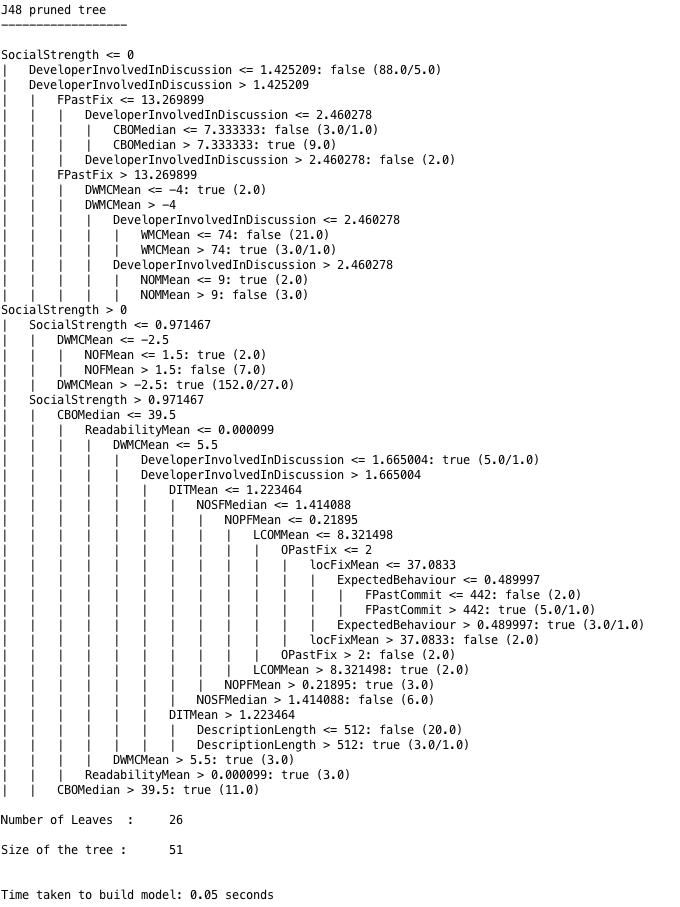
\includegraphics[width=0.5\textwidth]{j48.png}
  \caption{Weka J48 tree}\label{fig:j48}
\end{figure}




\subsection{Replication Package}
% A link to a zip file containing all the data and \emph{R} scripts used to run the study. The zip file must contain a $\mathtt{README.txt}$ file explaining the data and the scripts.
The prediction tool is implemented in Java and you can find it on  \href{https://github.com/talalelafchal/ReopenBugPrediction/tree/master/BugReopenPredictor}{Github}\footnote{https://github.com/talalelafchal/ReopenBugPrediction/tree/master/BugReopenPredictor} . In the output folder you can find all Weka's file and all csv files where we calculate the \emph{average, median} and \emph{standard deviation}. You also find a $\mathtt{README.txt}$ file explaining the data.

\section{Results Discussion}
% Discussion of the achieved results. Tip: define a subsection for each research question; conclude the results discussion for each research question by explicitly answering it.
  Before discussing the results we have to mention that two factors affect the utility of our tool: 
  
  \begin{itemize}
  \item it needs to be able to flag a substantial number of the reopened bugs.
  \item  it should not wrongly flag too many bugs as reopened bugs when they are not.
  \end{itemize}

  These factors are captured in the \emph{precision} and \emph{recall} metrics. A high precision and recall means that the number of wrongly flagged bug reports is low and that most of the reopened bugs are flagged.\cite{Shihab:wcre}\\

  In the three sampling techniques we have a low \emph{standard deviation} value, which confirm the fact that our random sampling is not affecting the result. The three techniques give us three different results, so let's discuss the impact of each of them.

	
	\subsection {Undersampling 100-100} As we explained before in this sampling method we have the same set size, so we have 91 reopened bug samples and 91 not reopened samples. The \emph{accuracy precision} and \emph{recall} are $66\%$ for predicting a $\overline{reopened Bug}$, and they are $66\%$ for predicting a $reopenedBug$. We can conclude that 91 samples are not enough to have a good confidence in predicting a bug reopening, since $66\%$ is not a high number that allows us to have a good confidence. 
	
	
	\subsection {Undersampling 100-200} In this sampling method we have 91 reopened bug samples and 182 not reopened samples. As we can see in Table \ref{table:Undersampling200} the confidence in predicting a $\overline{reopened Bug}$ is higher now, we have $71.8\%$ of \emph{precision} and $84.9\%$ of \emph{recall}, but on the other hand we still have low \emph{accuracy} $67.6\%$, and our confidence in predicting a $reopenedBug$ is bad, we have $52\%$  \emph{precision} and $33.3\%$ \emph{recall}. In this study we are more interested in $reopenedBug$ prediction, and this result doesn't allow us to have a good confidence. A reason for having such a result can be the fact that the number of reopened bug samples is small.
	
	\subsection{Oversampling 100-100} In this sampling method we create 91 artificial reopened bug samples; so now we have 182 reopened and not reopened bug samples. Increasing the number of samples changes drastically the result, now we have a high confidence in predicting a $reopenedBug$.
	As we can see in Table \ref{table:Oversampling} we have $78.8\%$ \emph{accuracy} and the $\overline{reopened Bug}$ \emph{F-Measure} is $78.1\%$ and $79.4\%$ for ${reopened Bug}$. This result allows us to have a high confidence in our prediction, and this is what we are looking for in our research.


\section{Threats to Validity}
%Discuss the threats that could affect the validity of the reported results.
Now we discuss possible threats to validity of our study. One big problem that we faced was to map the bug issue to the fix commit, Table \ref{tab:linked} shows that we were able to map only $40\%$ of the closed bug issues to their fixing commits, which means that we are loosing $60\%$ of important data which can change our prediction results.\\
The mapping technique that we used can add some bias, since we assume that if the developer who closed the bug issue did a commit before closing the issue, this commit must be the fixing commit.\\
Another possible bias can be in the way we interpreted the fact that the \emph{step to reproduce the bug} and the \emph{expected behavior} are present in the bug description. It is possible that key words which we try to find are not enough, and maybe there is a better approach.\\
It is difficult to generalize our work since we have analyzed only 3 projects, and all of them are Java projects.\\ It is probable that the bug prediction can be related to the programing language. We didn't investigate this possibility since we assumed that programming language feature is not one of the main reason to reopen a bug, and therefore we analyzed only Java projects. 




\section{Conclusion and Future Work}
% Summarize your findings, highlight ideas for future work (No more than one column).
In this paper we extract 28 features from different aspects as the developer experience and the code quality and the textual report description, to predict a reopened bug. We achieve $77.2\%$ of \emph{precision} and $81.8\%$ \emph{recall}. With such a confidence we can suggest the programmer to put more effort, and to add more test cases since this bug issue is a good candidate to be reopened in the future.\\
As a future work we can analyze more repositories to gather more reopened bug issues, since more we have better is our prediction. We can also try other techniques to extract the features, and we can analyze repositories written in different programing language than Java.


\bibliographystyle{ACM-Reference-Format}
\bibliography{bibliography}

\end{document}
